\documentclass{article}
\usepackage{latexsym}
\usepackage{amsmath}
\usepackage[a4paper]{geometry}
\usepackage{fullpage}
\usepackage{hyperref}
\usepackage{booktabs}
\usepackage{graphicx}
\usepackage{tikz}
\usepackage{xcolor}
\usepackage[export]{adjustbox}
\usepackage{comment}
\usepackage{subcaption}
\usepackage[style=iso]{datetime2}
\usepackage{cleveref}
\usepackage{listings}

%\usetikzlibrary{calc}
\usetikzlibrary{arrows,positioning} 
\tikzset{
    %Define style for course boxes
    courseboxv/.style={
           rectangle,
           draw=blue!50!black, very thick,
           fill=blue!10,
           minimum height=8cm,
           minimum width=4cm,
           text width=3.9cm,
           text centered,
           font=\bfseries\sffamily},
    courseboxh/.style={
           courseboxv,
           minimum height=4cm,
           minimum width=8cm,
           text width=7.9cm},
    courseboxhh/.style={
           courseboxh,
           minimum height=4cm,
           minimum width=16cm,
           text width=15.9cm}
}
\def\frameseparation{1.5cm}
\def\scalingfactor{.8}

\newcommand{\secref}[1]{Section~\ref{sec:#1}}
\newcommand{\secreff}[2]{Sections \ref{sec:#1} and \ref{sec:#2}}
\newcommand{\eqnref}[1]{Equation~\eqref{eq:#1}}
\newcommand{\eqnreff}[2]{Equations \eqref{eq:#1} and \eqref{eq:#2}}
\newcommand{\eqnrefff}[3]{Equations \eqref{eq:#1}, \eqref{eq:#2} and \eqref{eq:#3}}
\newcommand{\figref}[1]{Figure \ref{fig:#1}} 
\newcommand{\figreff}[2]{Figures \ref{fig:#1} and \ref{fig:#2}}
\newcommand{\figrefff}[3]{Figures \ref{fig:#1}, \ref{fig:#2} and \ref{fig:#3}}
\newcommand{\tabref}[1]{Table~\ref{tab:#1}}
\newcommand{\tabreff}[2]{Tables~\ref{tab:#1} and \ref{tab:#2}}
\newcommand{\tabrefff}[3]{Tables~\ref{tab:#1}, \ref{tab:#2} and \ref{tab:#3}}

\def\year{2024--2025}
\title{EITA65 Design of Systems for Digital Transformation\\\year}
%\title{EITA65 Digitalisering -- realisering och systemdesign med användarperspektiv\\\year}
\author{\huge Multi-Drone System\\Drone Project -- Part 5}
%\\Version \DTMnow}
%\date{}

\begin{document}
\newgeometry{left=2.5cm,right=2.5cm,bottom=1.5cm}% for placing course schematic lower on first page
\clearpage\maketitle
\thispagestyle{empty}% to remove page numbering on first page

\begin{itemize}
\item 
\includegraphics[width=3mm]{person.png}
\includegraphics[width=3mm]{person.png}
\includegraphics[width=3mm]{person.png}
\includegraphics[width=3mm]{person.png} In this project, you will work together in groups  of 3 or 4.  
\item You will not get detailed step-by-step instructions. Figuring out how to reach the goal is part of the project. (being a collaborative doer)
\item The results of this project part will be used in the next, so document your work.
\end{itemize}

\vspace{.1cm}
\begin{center}
\begin{tabular}{l}
\toprule[1.5pt]
\parbox{0.8\linewidth}{
\vspace{.2cm}{\Large Learning goals:}
\begin{itemize}
    \item Building a multi-drone capable system,
    \item Improved Redis skills; how to construct Redis queries for writing and reading data,
    \item Practice active collaboration with your group members.
\end{itemize}}\\
\bottomrule[1.5pt]
\end{tabular}
\end{center}
\vfill
% \begin{center}
% 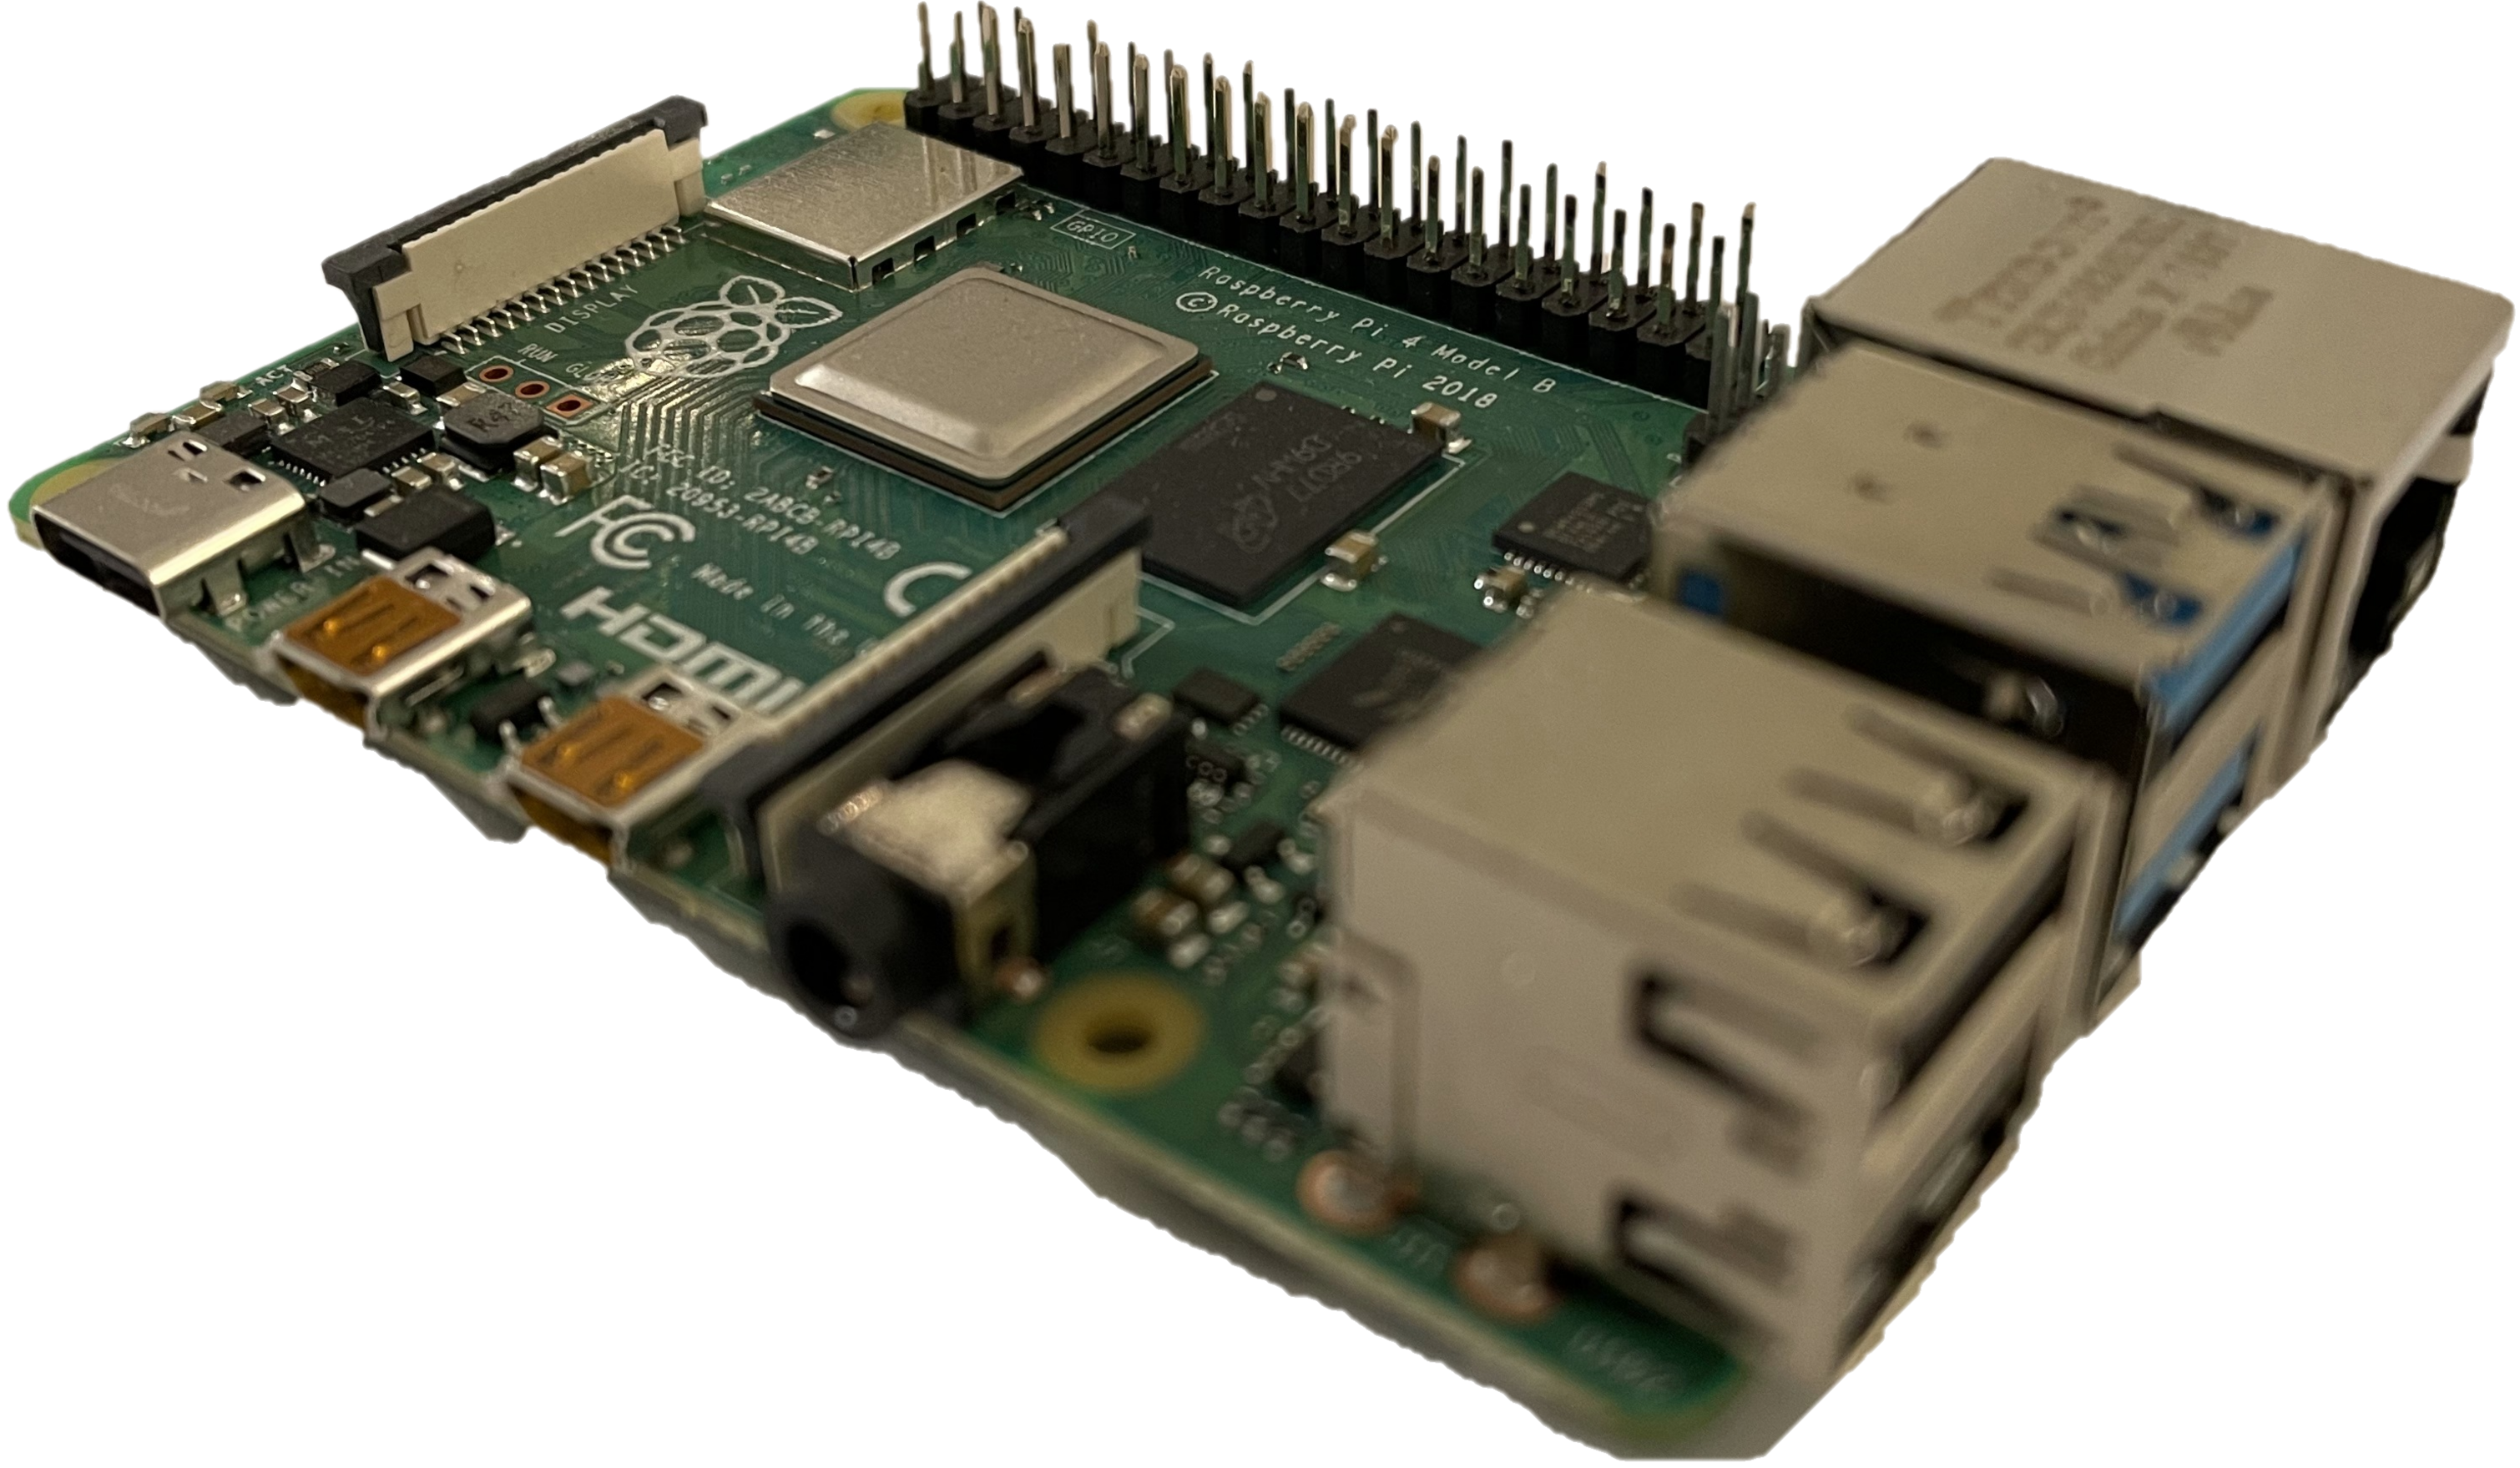
\includegraphics[width=120mm]{rpi4_no_bg.png}
% \end{center}
%\vspace{0.5cm}
\begin{center}
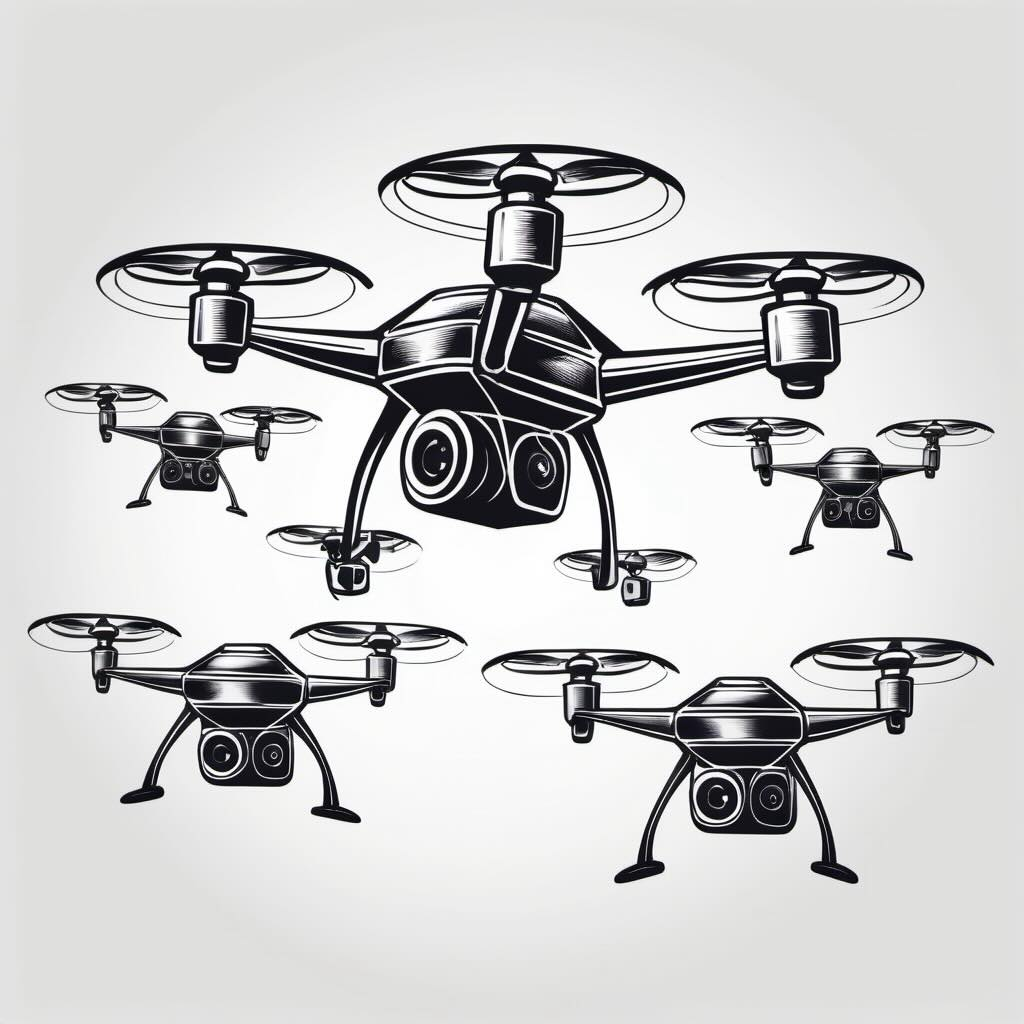
\includegraphics[width=90mm]{swarm.jpg}
\end{center}

\begin{comment}
\begin{center}
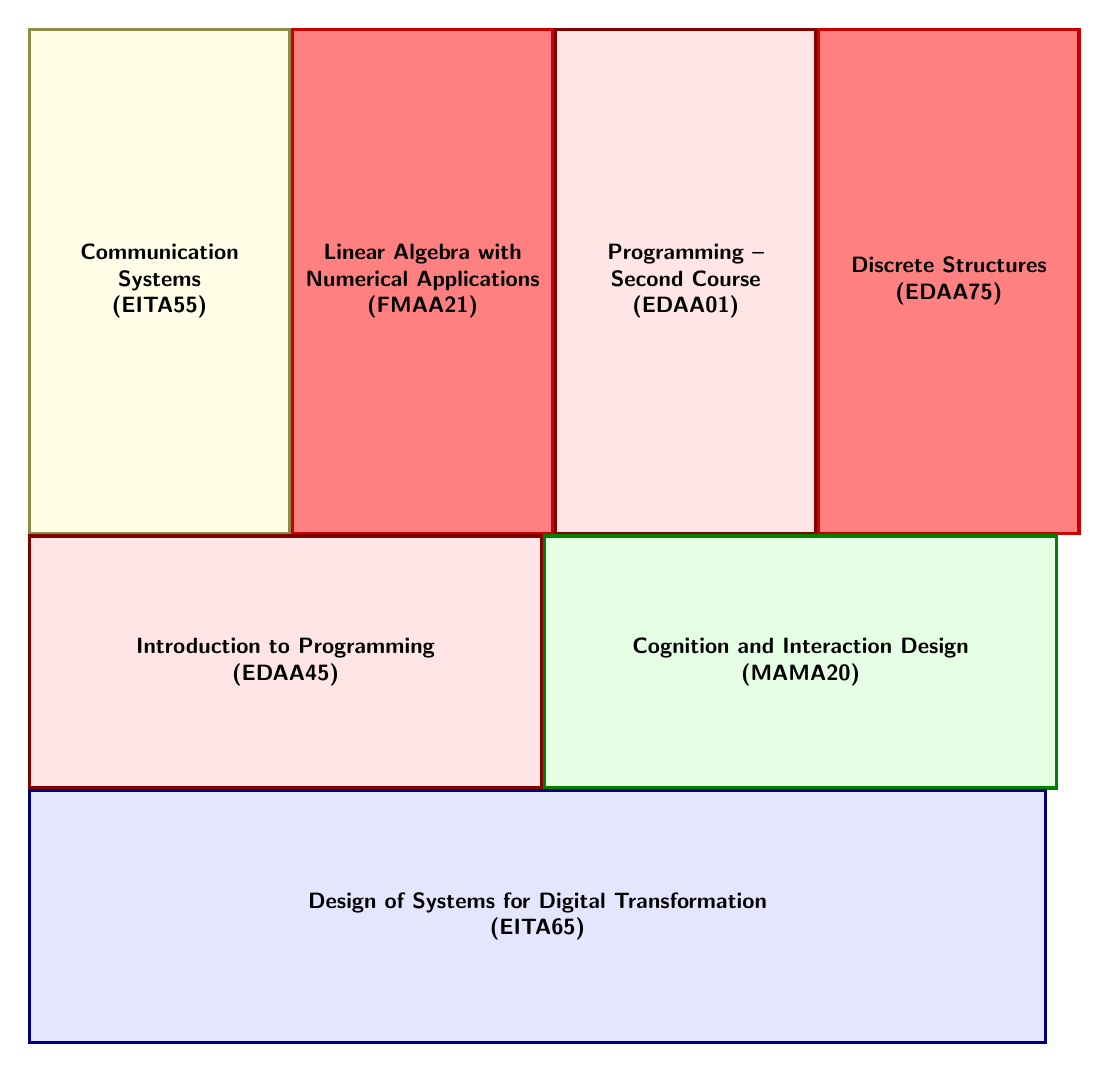
\begin{tikzpicture}[>=latex, node distance=0cm,scale=\scalingfactor,every node/.style={scale=\scalingfactor}]
\node[courseboxv, draw=yellow!50!black, fill=yellow!10] (EITA55) {Communication Systems\\(EITA55)};
\node[courseboxv, draw=red!80!black, fill=red!50, anchor=west] (FMAA21) at (EITA55.east){Linear Algebra with Numerical Applications\\(FMAA21)};
\node[courseboxv, draw=red!50!black, fill=red!10, anchor=west] (EDAA01) at (FMAA21.east){Programming -- Second Course\\(EDAA01)};
\node[courseboxv, draw=red!80!black, fill=red!50, anchor=west] (EDAA75) at (EDAA01.east){Discrete Structures\\(EDAA75)};
%\node[courseboxh, preaction={clip, postaction={fill=red!10, draw=red!50!black, line width=2mm}}, anchor=north west] (EDAA45) at (EITA55.south west){Introduction to Programming\\(EDAA45)};
\node[courseboxh, draw=red!50!black, fill=red!10, anchor=north west] (EDAA45) at (EITA55.south west){Introduction to Programming\\(EDAA45)};
%\node[courseboxh, draw=green!50!black, fill=green!10, anchor=west] (MAMA20) at (EDAA45.east){Cognition and Interaction Design\\(MAMA20)};
\node[courseboxh, draw=green!50!black, fill=green!10, right=of EDAA45] (MAMA20) {Cognition and Interaction Design\\(MAMA20)};
\node[courseboxhh, anchor=north west] (EITA65) at (EDAA45.south west){Design of Systems for Digital Transformation\\(EITA65)};
%\node[anchor=south east, inner sep=2pt, font=\bfseries\sffamily\scriptsize] at (EDA625.south east) {Helsingborg};
%\path[->,draw=black,dotted,thick] (EIT060.east) -- (EITF05.west);
%\path[->,draw=black,dotted,thick] (EIT060.south) -- (EITN50.north);
%\path[->,draw=black,dotted,thick] (EITF05.south) -- (EITN41.north);
%\draw[draw=blue!50!black, very thick] ($(EIT060.north west)+(-\frameseparation,\frameseparation)$) rectangle ($(EDA625.south east)+(\frameseparation,-\frameseparation)$);
\end{tikzpicture}
\end{center}
\end{comment}

\restoregeometry
\newpage


\section{Introduction}
In this part, you will extend the system you built in the previous lab to a more complex one that consists of two or more drones for delivery tasks. When the system is completed, you will be able to see multiple drones on the same map, with different status labels.

There are some things that you need to know before you go to the lab. This is a group task, so you will need to work in your group with all the other members. You also need to know the following items in advance:
\begin{itemize}
    \item  You will need to use the local area network you set up in the previous assignment -- the switch will be used once again.
    \item Each group needs to bring at least {\bf three} Raspberry Pis to the lab.
    \item One of the Raspberry Pis will need to run the server and the other Pis will simulate one drone each. If you wish to, you can replace the Server Pi with your own laptop, but make sure that they are all connected to the LAN you have built.
    \item You will, as before, not be handed step-by-step introductions, but please utilize Internet searches for knowledge as you encounter the need.
\end{itemize}

\section{Introduction to the System}
\subsection{Architecture of a two-drone system}
\begin{figure}
    \centering
    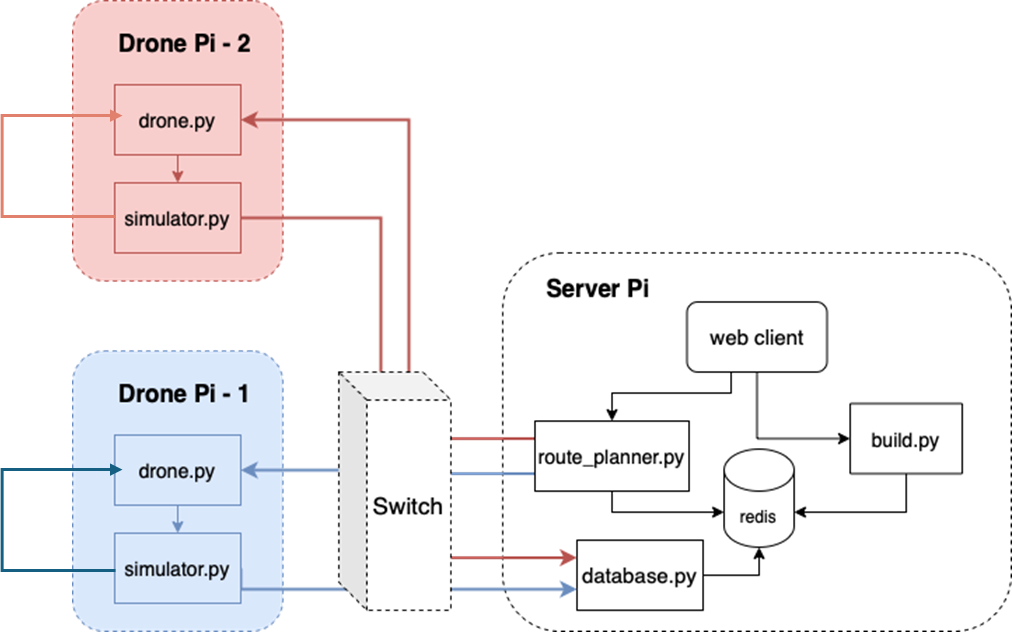
\includegraphics[width=\linewidth]{architecture.png}
    \caption{Two-drone system architecture.}
    \label{fig:sys}
\end{figure}
\Cref{fig:sys} illustrates the architecture of a two-drone system that you need to build. You can think of this illustration as being part of a system specification document. As you can see, you need to run all the servers on the Server Pi, and the drone simulator on each of the Drone Pis. You need to fork {\color{blue}{ \href{https://github.com/rogerhenriksson/InfoCom-Drone-5-Multi-drone_System}{this GitHub repository}}} and clone it on all the Raspberry Pis and run the scripts on the corresponding devices. It is suggested to fork the repository for each group and then use the same repository for all group members. Before you run the system, you need to fill in some missing code as indicated in the comments, as well as in this introduction. The majority of the coding tasks are on the server side, so you first need to make a sketch of the system all together and to distribute the coding tasks evenly. Intense collaboration is required in this lab.

Now let us take a look at each system component to see what work you need to do in order to complete the system.
\subsection{The Drone Pis}
\subsubsection{drone.py}
On each Drone Pi, you need to run a flask server (\verb!drone.py!) that listens to delivery requests sent from the route planner. Once the request has been received, it will invoke \verb!simulator.py! to run the delivery simulation. The functionalities you need to complete in this script are:
\begin{enumerate}
    \item You need to assign an ID to the Drone Pi. This ID should be unique for each Drone Pi that runs the script.
    \item Before you start listening for requests, you need to get the Pis current longitude and latitude to send to the Redis database on the server side. The longitude and latitude should be in OSM\cite{OSM} coordinates, so you need to either assign one manually or to create a text file and read the coordinate from there.
    \item To send the initial coordinates of the drone, you need to fill in the server's IP address and port number. Think about which server on the Server Pi that can update the drone information in the Redis database.
    \item As in LP 2, to invoke the simulator, you need to pass the arguments of \verb!current_coords!, \verb!from_coords! and \verb!to_coords!. The \verb!from_coords! and \verb!to_coords! values can be extracted from the request, but you need to find \verb!current_coords! on your own. But you cannott read it from the Redis server, since it is running on a different Raspberry Pi. Find a way to keep track of your own location on the Drone Pi. Hint : See task \ref{t2} in the next paragraph for simulator.py, you will use the same file.
\end{enumerate}

\subsubsection{simulator.py}
This script simulates the drone moving from \verb!current_location! to \verb!from_location!, and \verb!from_location! to \verb!to_location!, and updates the drone's real-time coordinates to the server while moving. This script is invoked by \verb!drone.py!, so you don't need to run it separately. You have two tasks when modifying this scripts:
\begin{enumerate}
    \item Fill in the database server URL in the script, so that you can update the coordinates to the Redis database running on the Server Pi.
    \item\label{t2} The simulator moves the drone and stops when the drone arrives at \verb!to_location!. You can save the final coordinates of the drone to a text file, so that the drone knows where it is and can start from this location as \verb!current_location! for the next delivery. Hint : You can use the open() function \cite{open}
\end{enumerate}

\subsection{The Server Pi}
The system architecture on the Server Pi is the same as in previous labs, but the functionality needs to be modified so that the server can handle information about multiple drones as well as matching tasks to drones and displaying the real-time statuses of all drones on the map.

\subsubsection{build.py}
This is the webserver that hosts the HTML file containing the map. The HTML page frequently generates requests to the server to ask for the latest information about each drone in order to update and display it on the map. These requests are handled by route \verb!/get_drones!. To respond to a request, the webserver needs to read all the relevant information from the Redis server. Package it in some way and then send the information package as a response. You need to fill in the following to complete the functionality:
\begin{enumerate}
    \item Put in the correct address of the Redis server.
    \item Read the information about all drones from the Redis server including the Drone ID, longitude, latitude and status ('busy' or 'idle') for each drone.
    \item Put the information in a nested dictionary. The client will only accepts JSON responses (see \cite{json}) in a specific format, so the dictionary needs to have the same format as the example given in the code comments(see source code build.py).
    \item The longitude and latitude in the response should be SVG values, but you will get OSM values from the database. Thus, before entering these data into the response dictionary, use the \verb!translate()! function to convert OSM coordinates to SVG coordinates.
\end{enumerate}

\subsubsection{database.py}
The database server listens for requests from drones, and incoming requests contain all (some) information sent by a specific drone. The request data are stored as a JSON file and resolved into the dictionary \verb!drone!. The dictionary contains ID, longitude, latitude and status of the drone that sends the requests. All the values need to be stored in the database properly, and the database needs to be updated when a request arrives (providing new status information for a drone). Other than the values in the dictionary, the IP address of the drone also needs to be stored in the database, so that the router planner can find and contact the drone in the network.

\subsubsection{route\_planner.py}
As in previous labs, the route planner gets the addresses you input on the webpage, searches for the OSM coordinates of the input addresses and sends the coordinates to a drone. Since, in this system, you have more than one drone, an additional task of the route planner is to find a drone that is available (not busy with a delivery mission), and send the delivery request to the available drone. You need to complete the task of finding an available drone and send the job request to the drone:
\begin{enumerate}
    \item Put in the correct address of the Redis server.
    \item Find an available drone in the Redis database by first searching for the status of all drones in the database server. If the drone status is 'busy', its not available. If the status is 'idle', the drone is available.
    \begin{itemize}
        \item If there is no drone available, you need to return the message {\textsc{`No available drone, try later'}} as response.
        \item If there is an available drone, get the IP address of the drone in the database, compose the URL with the IP and send coordinates in the HTTP request to the drone. An example of how to send such a request is given in the code. After sending the request, you must return the message\textsc{`Got address and sent request to the drone'} as response.
    \end{itemize}
\end{enumerate}

When you have finished all tasks, you should be able to run the system following the instructions in the \texttt{README.md} file in the repository. Show the TA your completed system when you have finished it.

\vspace{1cm}
\begin{center}
\huge Good luck!
\end{center}

\begin{thebibliography}{10} \bibliographystyle{plain}

\bibitem{json} JavaScript Object Notation (JSON) -- Wikipedia, \url{https://en.wikipedia.org/wiki/JSON}, last accessed on 2024-01-20.

\bibitem{OSM} OpenStreetMap, \url{https://www.openstreetmap.org/#map=14/55.7059/13.2005}, last accessed on 2024-01-20.

%\bibitem{try} Try and Except in Python, \url{https://pythonbasics.org/try-except/}, last accessed on 2024-01-25.

\bibitem{open} Python open() function, \url{https://www.geeksforgeeks.org/writing-to-file-in-python/}, last accessed on 2024-01-20.

\end{thebibliography}

\end{document}
